\documentclass{article}
\usepackage[T1]{fontenc}
\usepackage{lmodern}
\usepackage[polish]{babel}
\usepackage{graphicx}
\usepackage{float}
\usepackage{hyperref}
\usepackage{amsmath} 
\usepackage{multicol}
\usepackage{listings}
\usepackage{tikz} % pgf package
\usetikzlibrary{shapes.multipart}

\usepackage[a4paper, margin=2.54cm]{geometry}

\lstdefinestyle{siec}{
    basicstyle=\ttfamily\footnotesize,
    frame = tb,
    title={Struktura sieci},
    backgroundcolor=\color{gray!10},
}

\title{Sprawozdanie z projektu ze Sztucznej Inteligencji \\ 
Porównanie metod uczenia maszynowego \\ 
w problemie MNIST i jego pochodnych}
\author{Filip Gołaś s188776 \\ Damian Jankowski s188597 \\ Mikołaj Storoniak s188806}

\begin{document}

\maketitle

\tableofcontents

\section{Opis problemu}

Celem projektu było zbudowanie i porównanie różnych
modeli uczenia maszynowego w problemie klasyfikacji
obrazów z bazy MNIST. Korzystaliśmy głównie z bazy
danych \textbf{MNIST-784}, która zawiera 70 tysięcy obrazów
cyfr napisanych ręcznie. Każdy obraz jest w skali
szarości i ma rozmiar 28x28 pikseli. Każdy piksel
jest reprezentowany przez liczbę całkowitą z zakresu
od 0 do 255, która określa jasność piksela. Dodatkowo
każdy obraz ma przypisaną etykietę, która określa
jaką cyfrę przedstawia obraz.

\begin{figure}[H]
    \centering
    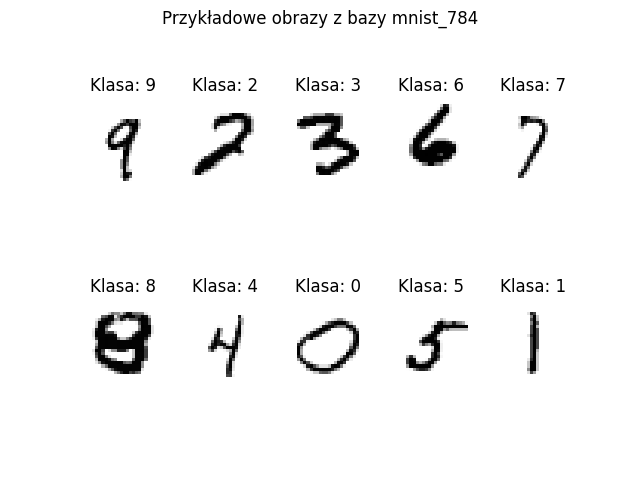
\includegraphics[width=0.8\textwidth]{baza_mnist_784.png}
\end{figure}

Zdecydowaliśmy się również na wykorzystanie bazy
danych \textbf{Fashion-MNIST}, która podobnie jak poprzednia, zawiera
70 tysięcy obrazów o rozmiarze 28x28 pikseli, natomiast
każdy obraz przedstawia wybrane ubranie lub akcesorium.

\begin{figure}[H]
    \centering
    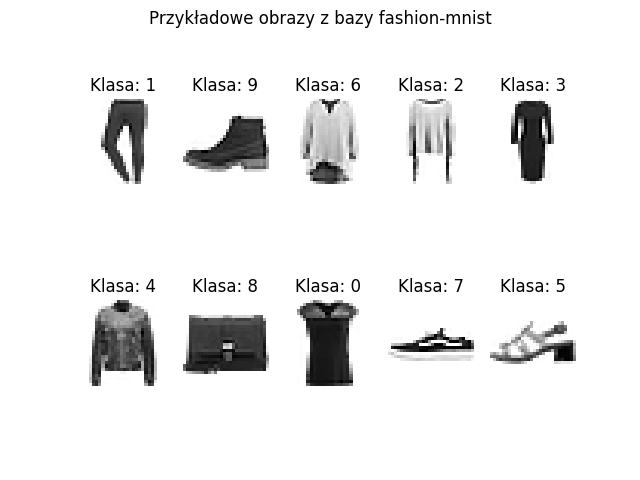
\includegraphics[width=0.8\textwidth]{baza_fashion_mnist.png}
\end{figure}

Opis klas w bazie danych Fashion-MNIST:

\begin{enumerate}
    \begin{multicols}{2}
        \centering
        \setcounter{enumi}{-1}
        \item T-shirt/top
        \item Trouser
        \item Pullover
        \item Dress
        \item Coat
        \item Sandal
        \item Shirt
        \item Sneaker
        \item Bag
        \item Ankle boot
    \end{multicols}
\end{enumerate}


\section{Opis porównanych modeli}

\subsection{Drzewa}
\subsubsection{Drzewo decyzyjne}
Drzewo decyzyjne jest modelem predykcyjnym wykorzystywanym w 
dziedzinie uczenia maszynowego i analizy danych. Jest to 
struktura drzewiasta, w której każdy węzeł reprezentuje 
test na jednej z cech, gałęzie reprezentują możliwe wyniki 
tego testu, a liście reprezentują etykiety lub wartości 
predykcyjne. Drzewo decyzyjne może być wykorzystane 
zarówno do klasyfikacji, jak i do regresji.

Podczas konstrukcji drzewa decyzyjnego, 
algorytm dokonuje podziału zbioru danych 
na podzbiory na podstawie wybranych cech. 
Celem jest jak najlepsze rozdzielenie danych, 
aby w każdym podzbiorze dominowała jedna klasa 
lub aby zminimalizować błąd predykcji dla zmiennych 
ciągłych w przypadku regresji.

Drzewa decyzyjne posiadają wiele zalet, takich jak 
prostota interpretacji, zdolność do obsługi zarówno 
danych kategorycznych, jak i numerycznych, oraz efektywność 
obliczeniowa w przypadku dużych zbiorów danych. Jednakże, 
mogą być podatne na przetrenowanie, co oznacza, że mogą zbyt 
dobrze dopasować się do danych treningowych i słabo generalizować na nowe dane.

\subsubsection{Las losowy}
Las losowy (ang. Random Forest) jest złożonym modelem 
predykcyjnym, który opiera się na kombinacji wielu drzew decyzyjnych. 
Polega na budowie wielu drzew decyzyjnych na podstawie 
różnych losowych podzbiorów danych treningowych, a 
następnie łączeniu ich wyników w celu uzyskania ostatecznej 
predykcji. Każde drzewo w lesie losowym jest budowane 
niezależnie od pozostałych, a wyniki są łączone w procesie 
głosowania lub uśredniania.

Las losowy ma wiele zalet, w tym wysoką dokładność 
predykcji, zdolność do obsługi zarówno danych 
kategorycznych, jak i numerycznych, oraz odporność 
na przetrenowanie. Dodatkowo, las losowy może dostarczać 
ważność cech, co oznacza, że można ocenić, które cechy 
mają największy wpływ na predykcje.

Las losowy znajduje zastosowanie w wielu dziedzinach, 
takich jak klasyfikacja obrazów, przetwarzanie 
języka naturalnego, analiza danych medycznych itp. 
Jest to popularny model ze względu na swoją elastyczność 
i dobrą wydajność nawet w przypadku dużych zbiorów danych.

\subsection{Sieci neuronowe}
Sieć neuronowa jest modelem statystycznym czerpiącym inspirację z natury i 
działania układów nerwowych żywych organizmów.
Modele te są stosowane zarówno do problemów regresji (aproksymacji) jak i klasyfikacji poprzez nauczanie nadzorowane.

Podstawową składową każdej sieci neuronowej jest neuron, który może być reprezentowany 
jako funkcja wielu parametrów zwracająca dyskretną wartość
prawda lub fałsz. Choć jeden neuron nie jest w stanie opisać złożonych modeli, 
dużo większe możliwości mają sieci neuronowe zbudowane z wielu neuronów
połączonych w warstwy w taki sposób, że wynik jednej warstwy służy jako parametry kolejnej.

% TU WSTAWIĆ ILUSTRACJĘ WARSTW PRZEKAZUJĄCYCH SOBIE PARAMETRY

Poprzez odpowiednie ustawienie współczynników funkcji w neuronach jesteśmy w 
stanie zamodelować zależności dużo bardziej złożone niż te możliwe do opisania jedną
prostą funkcją wielu parametrów.

\subsubsection{Wielowarstwowy perceptron}

W praktyce w sieciach neuronowych neurony są zastąpione perceptronami, które od neuronów 
różnią się tym, że są funkcjami w dziedzinie rzeczywistej.
Same warstwy neuronów również nie są reprezentowane jako zbiory obiektów typu neuron. 
Operacja przechodzenia danych wejściowych przez kolejne warstwy sieci
zwana propagacją w przód może być zrealizowana w każdej warstwie poprzez proste mnożenie macierzy

\begin {equation}
    S = X \times W
\end{equation}
gdzie:
\begin{itemize}
    \item $X$ jest macierzą $(n, 1)$ parametrów będących danymi 
    wejściowymi sieci w przypadku warstwy pierwszej (wejściowej), 
    lub wartości zwróconych przez poprzednią warstwę w sieci
    \item $W$ jest macierzą $(m, n)$ współczynników funkcji opisujących perceptrony, 
    w której każdy wiersz opisuje jeden perceptron, 
    a każda kolumna odpowiada wartości współczynnika tego perceptronu dla danego parametru 
    z wektora wejściowego warstwy
    \item $S$ jest macierzą wynikową warstwy $(1, m)$ zawierającą wartości zwrócone przez 
    funkcje opisujące perceptrony tworzące tę warstwę
\end{itemize}

Następnie należy zdecydować kiedy uznamy dany neuron za pobudzony. Do tego zadania 
stosuje się funkcje aktywacji, których dobór jest niezwykle ważny
i może łatwo zadecydować o użyteczności sieci.

\begin{equation}
    f(S) = Z
\end{equation}

\begin{itemize}
    \item $f(\cdot)$ jest wybraną funkcją aktywacji, która powinna być 
    różniczkowalna by możliwe było użycie jej w propagacji wstecz
    \item $S$ jest macierzą wynikową $(1, m)$ warstwy
    \item $Z$ jest macierzą $(1, m)$, w której każdy element jest intensywnością pobudzenia danego neuronu
\end{itemize}

Aby korzystać z sieci neuronowych do opisywania skomplikowanych modeli 
statystycznych nie możemy ręcznie decydować o wartościach parametrów w warstwach. 
Byłoby to niezwykle ciężkie o ile nie niemożliwe w sposób analityczny. 
Zamiast tego sieci neuronowe poddaje się trenowaniu.

Proces trenowania sieci neuronowej nazywany jest propagacją wstecz. Gdy 
przeprowadzimy proces propagacji w przód dla sieci z wartościami współczynników
o wartościach losowych o dowolnym rozkładzie jesteśmy w stanie poprawić 
je stosując wybraną różniczkowalną funkcję straty i znając wartości pożądane. Dzieje się to 
w najprostrzym przypadku poprzez metodę spadku po gradiencie, którą można 
opisać macierzowo dla całej warstwy neuronów jako:

\begin{equation}
    W_1 = W_0 - \eta \times \frac{\partial E}{\partial Z}
\end{equation}
gdzie:
\begin{itemize}
    \item $W_0$ jest macierzą $(m, n)$ współczynników perceptronów warstwy, a $W_1$ jest jej nową postacią
    \item $\eta$ jest współczynnikiem $learning rate$ kontrolującym tempo uczenia
    \item $\frac{\partial E}{\partial Z}$ jest pochodną z sygnału błędu po 
    macierzy wynikowej $S$ danej warstwy. Sygnał błędu w przypadku ostatniej warstwy (wyjściowej) jest
    gradientem funkcji błędu macierzy wynikowej, w przypadku reszty warstw 
    jest on sygnałem błedu pochodzącym z poprzednio aktualizowanej w procesie propagacji wstecz warstwy
    wyznacznym poprzez:
    \begin{equation}
        E_1 = -\frac{\partial E_0}{\partial S}
    \end{equation}
    gdzie:
    \begin{itemize}
        \item $E_0$ jest sygnałem błędu zwracanym przez daną warstwę
        \item $\frac{\partial E}{\partial S}$ jest pochodną cząstkową z sygnału błedu, 
        który otrzymała ta warstwa od warstwy poprzedniej w procesie propagacji wstecz, lub w przypadku warstwy
        wyjściowej gradientem funkcji straty dla macierzy wyjściowej tej warstwy
    \end{itemize}
\end{itemize}

\subsubsection{Sieć konwolucyjna}
Sieć konwolucyjna jest odmianą sieci neuronowej, 
w której stosuje się warstwy konwolucyjne. W takich 
warstwach każdy neuron zamiast nakładać na zbiór parametrów 
funkcję, nakłada na nie filtr, którego wagi są współczynnikami 
neuronu. Filtr może być w postaci wektora, małej macierzy kwadratowej, 
lub kilku macierzy w zależności od tego czy interpretujemy dane wejściowe 
jako wektor, powierzchnię czy przestrzeń punktów. Odpowiednio wytrenowana 
sieć konwolicyjna jest w stanie skutecznie wykrywać i wzmacniać poprzez 
nakładanie filtrów istotne cechy danych, które następnie mogą posłużyć 
jako wejście dla warstwy zwykłych perceptronów, które dzięki temu wyszczególnieniu 
kluczowych cech dużo skuteczniej poradzą sobie w rozwiązaniu zadania.

Poza warstwami konwolucyjnymi w sieciach konwolucyjnych stosuje się 
często Max Pooling. Nie jest to warstwa neuronowa, lecz procedura 
przetwarzająca obrazy utworzone przez warstwy konwolucyjne zmniejszająca 
rozmiar tworzonych przez sieć obrazów poprzez wstawianie w miejsce każdego 
okna $n \times n$ wartość maksymalną z tego okna.

Kolejne udoskonalenie modelu polegało na dodaniu procedury Dropout jako 
jednej z warstw sieci. Dropout ustawia z pewnym prawdopodobieństwem pojedyncze 
wartości mu przekazane na 0 w ten sposób wykluczając pewne obserwacje sieci z 
rezultatu i zmniejszając szansę na przeuczenie sieci, co skutkowałoby doskonałym 
klasyfikowaniem danych, na których model był uczony, lecz nie radzeniem sobie 
zupełnie z nowymi nie widzianymi przez niego danymi.
\subsubsection{Sieć grafowa}

\subsubsection{Konwolucyjna sieć transferowa}
Z racji, że różne zadania klasyfikacji obrazów nie różnią się od siebie tak drastycznie jak 
mogłoby się wydawać, popularnym sposobem na tworzenie bardzo dokładnych 
klasyfikatorów jest korzystanie z sieci transferowych. Są to sieci konwolucyjne korzystające 
z wytrenowanej już wcześniej na innych problemach klasyfikacji warstw konwolucyjnych. 
Proces nauczania takiej sieci neuronowej jest o wiele prostszy, gdyż wytrenowania wymaga 
jedynie mała ilość nowych warstw, które zinterpretują wyniki juz gotowych i wytrenowanych 
w klasyfikacji obrazów warstw konwolucyjnych. W pierwszych etapach nauczania należy pominąć 
już wytrenowane warstwy konwolucyjne aby usprawnić ten proces. Gdy model jest już dostatecznie 
dobrze wytrenowany można odblokować trenowanie warstw konwolucyjnych, by przeprowadzić tzw. 
fine tuning, który pozwoli wyspecjalizować warstwy konwolucyjne w detekcji cech charakterystycznych dla danego problemu. 


\subsection{KNN - K Nearest Neighbours}
KNN jest modelem bezparametrycznego uczenia nadzorowanego. Jest to niezwykle prosty model,
 który nie wymaga procesu uczenia, jednak przypłaca to bardzo kosztowną predykcją.
Algorytm K Nearest Neighbours polega na obliczeniu odległości wektora danych wejściowych 
długości n traktowanego jako punkt w przestrzeni n wymiarowej i porównaniu go z każdym z 
pośród wektorów danych wejściowych dostarczonych modelowi w ramach danych treningowych, 
które to model zapamiętał. Punkty z pośród danych treningowych wraz z ich etykietami 
następnie są sortowane rosnąco wedle ich odległości od danej wejściowej, której 
klasyfikację przeprowadza model. Następnie dopierane jest K pierwszych z pośród 
punktów, których to odległość od klasyfikowanego punktu jest najniższa i zliczane 
są wystąpienia różnych typów etykiet pośród wybranych K punktów. Ta etykieta, 
która pośród nich powtarza się najczęściej jest odpowiedzią modelu na zadanie klasyfikacji.

\section{Opis realizacji zadania}

\subsection{Drzewo decyzyjne}

Wykorzystując bibliotekę scikit-learn zaimplementowano model drzewa
decyzyjnego. W celu znalezienia najlepszych parametrów modelu losowo
wybierano wartości z pewnego przedziału i sprawdzano, dla których wartości
model osiąga najlepsze wyniki. Hiperparametry, które były brane pod uwagę to:

\begin{itemize}
    \item \textbf{max\_depth}: Określa maksymalną 
    głębokość drzewa decyzyjnego. 
    Głębokość drzewa to liczba poziomów w 
    drzewie, które składają się z węzłów 
    decyzyjnych i liści. Im większa wartość 
    max\_depth, tym bardziej skomplikowane 
    drzewo może zostać utworzone, co może 
    prowadzić do bardziej dopasowanego modelu. 
    Jednak zbyt duża wartość max\_depth może 
    prowadzić do przeuczenia (overfittingu) modelu.
    \item \textbf{max\_features}: Określa maksymalną
    liczbę cech, które należy wziąć pod uwagę
    przy każdym podziale węzła. Do wyboru są trzy opcje:
    \begin{itemize}
        \item \textbf{None}: max\_features = n\_features
        \item \textbf{sqrt}: max\_features = $\sqrt{n\_features}$
        \item \textbf{log2}: max\_features = $\log_2{n\_features}$
    \end{itemize}
    \item \textbf{min\_samples\_split}: Określa minimalną 
    liczbę próbek wymaganą do podziału węzła decyzyjnego. 
    Jeśli liczba próbek w węźle jest mniejsza niż 
    min\_samples\_split, to węzeł nie będzie podlegał 
    dalszemu podziałowi, co prowadzi do utworzenia 
    liścia. Niskie wartości min\_samples\_split mogą 
    prowadzić do przeuczenia modelu, podczas gdy 
    wysokie wartości mogą prowadzić do niedouczenia (underfittingu).
    \item \textbf{criterion}: Określa funkcję używaną 
    do pomiaru jakości podziału. Istnieją dwie do wyboru:
    \begin{itemize}
        \item \textbf{gini}: Współczynnik Giniego to miara
        nieczystości węzła, wyrażona jako suma prawdopodobieństw
        kwadratu prawdopodobieństwa każdej klasy.
        \begin{equation}
            G = 1 - \sum_{i=1}^{J}p_i^2
        \end{equation}
        gdzie: 
        \begin{itemize}
            \item $J$ - liczba klas
            \item $p_i$ - prawdopodobieństwo wystąpienia klasy $i$
        \end{itemize}
        Im niższa wartość współczynnika Giniego, tym lepszy podział.
        \item \textbf{entropy}: Entropia wyrażona równaniem:
        \begin{equation}
            E = -\sum_{i=1}^{J}p_i\log_2{p_i}
        \end{equation}
        Podobnie jak w przypadku współczynnika Giniego, im niższa
        wartość entropii, tym lepszy podział.
    \end{itemize}
    \item \textbf{splitter}: Określa strategię 
    wyboru podziału węzła. Do wylosowania jest
    jedna z dwóch opcji:
    \begin{itemize}
        \item \textbf{best}: Wybiera najlepszy podział.
        \item \textbf{random}: Wybiera najlepszy losowy podział.
    \end{itemize}

\end{itemize}

\subsection{Las losowy}

Podobnie jak w przypadku drzewa decyzyjnego, wykorzystując bibliotekę
scikit-learn zaimplementowano model, losując wartości
następujących hiperparametrów:

\begin{itemize}
    \item \textbf{n\_estimators}: Określa liczbę drzew decyzyjnych
    w lesie losowym.
    \item \textbf{max\_depth}: Określa maksymalną głębokość drzewa
    decyzyjnego.
    \item \textbf{max\_features}: Określa maksymalną liczbę cech,
    które należy wziąć pod uwagę przy każdym podziale węzła.
    \item \textbf{min\_samples\_split}: Określa minimalną liczbę
    próbek wymaganą do podziału węzła decyzyjnego.
    \item \textbf{min\_samples\_leaf}: Określa minimalną liczbę
    próbek wymaganą do utworzenia liścia.
    \item \textbf{criterion}: Określa funkcję używaną do pomiaru
    jakości podziału.
\end{itemize}

\subsection{Własna implementacja Wielowarstwowego perceptronu}

Z wykorzystaniem biblioteki numpy zaimplementowano model sieci neuronowej 
typu wielowarstwowy perceptron zgodny z powyższą teorią do bazy MNIST-784.

Architektura warstw stworzonej sieci wyglądała następująco:

% $$ 784 -> 512, sigmoid -> 256, sigmoid -> 128, sigmoid ->10, softmax $$

\begin{center}
    \begin{tikzpicture}[node distance=3cm, every node/.style={minimum height=0.8cm, minimum width=1.5cm}]
        \matrix[draw=none, column sep=0.5cm, row sep=0.6cm]{
            \node[rectangle, draw] (input) {784}; \\
            \node[rectangle, draw] (hidden1) {512}; \\
            \node[rectangle, draw] (hidden2) {256}; \\
            \node[rectangle, draw] (hidden3) {128}; \\
            \node[rectangle, draw] (output) {10}; \\
        };

        % Opisy kwadratów
        \node[above=0.3cm] at (input.north) {\textbf{Wejście}};
        \node[right=0.0cm] at (hidden1.east) {\tiny \textbf{Ukryta 1}};
        \node[right=0.0cm] at (hidden2.east) {\tiny \textbf{Ukryta 2}};
        \node[right=0.0cm] at (hidden3.east) {\tiny \textbf{Ukryta 3}};
        \node[below=0.3cm] at (output.south) {\textbf{Wyjście}};

        % Opisy etapów
        \node[below=0.3cm, right=0.0cm] at (input.south) {\tiny \textbf{sigmoid}};
        \node[below=0.3cm, right=0.0cm] at (hidden1.south) {\tiny \textbf{sigmoid}};
        \node[below=0.3cm, right=0.0cm] at (hidden2.south) {\tiny \textbf{sigmoid}};
        \node[below=0.3cm, right=0.0cm] at (hidden3.south) {\tiny \textbf{softmax}};

        \draw[->] (input) -- (hidden1);
        \draw[->] (hidden1) -- (hidden2);
        \draw[->] (hidden2) -- (hidden3);
        \draw[->] (hidden3) -- (output);
    \end{tikzpicture}
\end{center}

Za funkcję straty przyjęto funkcję Categorical Crossentropy, learning rate wynosił 0.01.
W trakcie trenowania nie korzystano żadnych mechanizmów nieomówionych 
w częsci teoretycznej w tym: batchingu czy przetwarzania danych wejściowych poza skalowaniem do zakresu $[0, 1]$.
\subsection{Wielowarstwowy perceptron Tensorflow Keras}

Z wykorzystaniem pakietu tensorflow.keras utworzono sieć neuronową o architekturze 
analogicznej do tej zaimplementowanej ręcznie. Zastosowano kilka zmian w postaci:

\begin{itemize}
\item Do propagacji wstecz zamiast stochastycznego schodzenia po gradiencie użyto algorytmu 
Adam będącego jego udoskonaleniem uwzględniającym momenty gradientu.
\item Zastosowano mechanizm batchingu, $batch_{size} = 128$
\end{itemize}

\begin{lstlisting}[style=siec]
    Model: "sequential"
    _________________________________________________________________
    Layer (type)                Output Shape              Param #
    =================================================================
    dense (Dense)               (None, 512)               401920

    dense_1 (Dense)             (None, 256)               131328

    dense_2 (Dense)             (None, 128)               32896

    dense_3 (Dense)             (None, 10)                1290
                                                                    
    =================================================================
    Total params: 567,434
    Trainable params: 567,434
    Non-trainable params: 0
    _________________________________________________________________
\end{lstlisting}

Proces uczenia sieci trwał 500 epok, a jego przebieg przedstawiono na poniższych wykresach:

\begin{figure}[H]
    \centering
    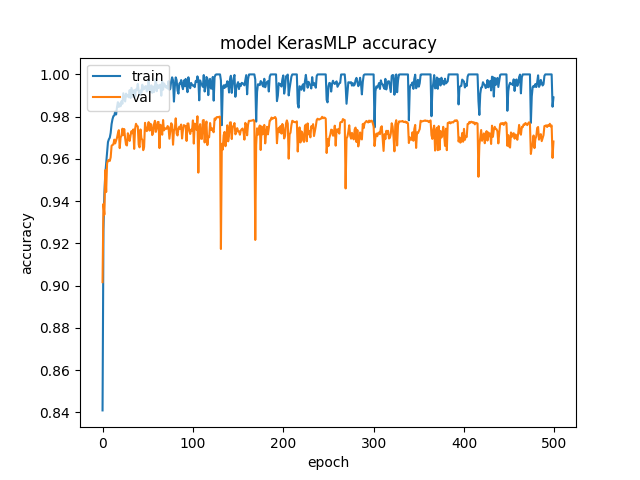
\includegraphics[width=0.6\textwidth]{../Saves/KerasMLP/KerasMLP_mnist_784_ep500_acc.png}
    \caption{Wykres dokładności w zależności od epoki}
\end{figure}

\begin{figure}[H]
    \centering
    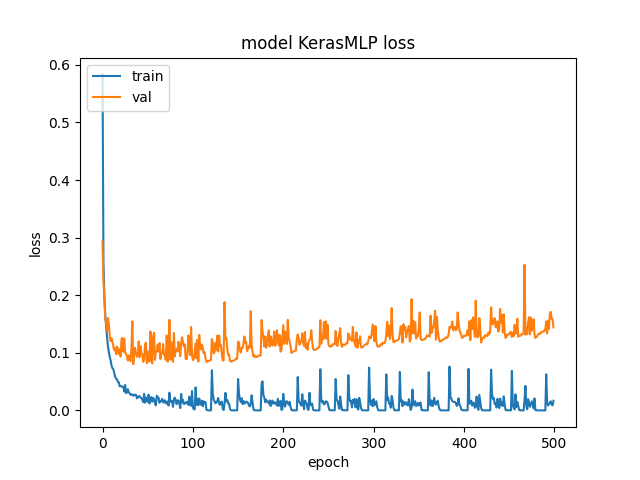
\includegraphics[width=0.6\textwidth]{../Saves/KerasMLP/KerasMLP_mnist_784_ep500_loss.png}
    \caption{Wykres wartości funkcji straty w zależności od epoki}
\end{figure}

\subsection{Sieć konwolucyjna Tensorflow Keras}

\subsubsection{Wersja podstawowa}
Sieć konwolucyjną zaimplementowano przy użyciu pakietu tensorflow keras. Wszystkie hiperparametry pozostały 
identyczne z wielowarstwowym perceptronem zaimplementowanym z użyciem tych samych bibliotek. 
Struktura sieci wyglądała następująco:

% $28x28-> 32x(3,3), relu -> maxPooling(2,2) 64x(3,3), relu -> maxPooling(2,2)->Flatten->Dropout(0.5) -> 10, softmax$

\begin{lstlisting}[style=siec]
    Model: "sequential"
    _________________________________________________________________
    Layer (type)                Output Shape              Param #   
    =================================================================
    conv2d (Conv2D)             (None, 28, 28, 32)        320       
                                                                    
    max_pooling2d (MaxPooling2D)  (None, 14, 14, 32)       0                                                                      
                                                                    
    conv2d_1 (Conv2D)           (None, 14, 14, 64)        18496     
                                                                    
    max_pooling2d_1 (MaxPooling  (None, 7, 7, 64)         0         
    2D)                                                             
                                                                    
    flatten (Flatten)           (None, 3136)              0         
                                                                    
    dropout (Dropout)           (None, 3136)              0         
                                                                    
    dense (Dense)               (None, 10)                31370     
                                                                    
    =================================================================
    Total params: 50,186
    Trainable params: 50,186
    Non-trainable params: 0
    _________________________________________________________________
\end{lstlisting}

Proces uczenia sieci trwał 500 epok, a jego przebieg przedstawiono na poniższych wykresach:

\begin{figure}[H]
    \centering
    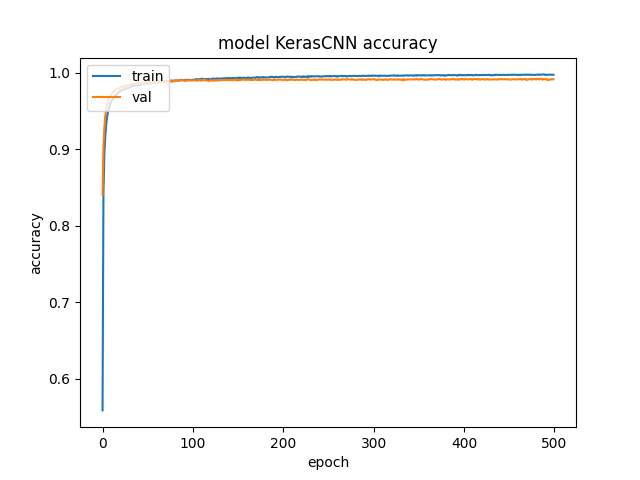
\includegraphics[width=0.6\textwidth]{../Saves/KerasCNN/KerasCNN_mnist_784_ep500_acc.png}
    \caption{Wykres dokładności w zależności od epoki}
\end{figure}

\begin{figure}[H]
    \centering
    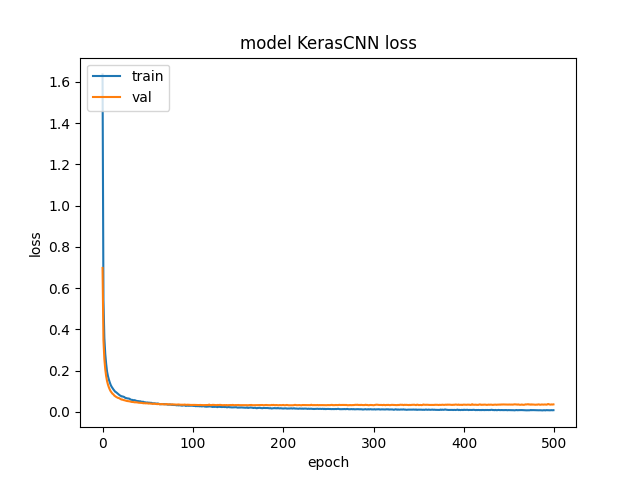
\includegraphics[width=0.6\textwidth]{../Saves/KerasCNN/KerasCNN_mnist_784_ep500_loss.png}
    \caption{Wykres wartości funkcji straty w zależności od epoki}
\end{figure}

\subsubsection{Wersja rozszerzona}

Dodatkowo dodano więcej warstw konwolucyjnych oraz warstw gęstych.

\begin{lstlisting}[style=siec]
    Model: "sequential"
    _________________________________________________________________
     Layer (type)                Output Shape              Param #   
    =================================================================
     conv2d (Conv2D)             (None, 24, 24, 32)        832       
                                                                     
     conv2d_1 (Conv2D)           (None, 20, 20, 32)        25600     
                                                                     
     batch_normalization (BatchN  (None, 20, 20, 32)       128       
     ormalization)                                                   
                                                                     
     activation (Activation)     (None, 20, 20, 32)        0         
                                                                     
     max_pooling2d (MaxPooling2D  (None, 10, 10, 32)       0         
     )                                                               
                                                                     
     dropout (Dropout)           (None, 10, 10, 32)        0         
                                                                     
     conv2d_2 (Conv2D)           (None, 8, 8, 64)          18496     
                                                                     
     conv2d_3 (Conv2D)           (None, 6, 6, 64)          36864     
                                                                     
     batch_normalization_1 (Batc  (None, 6, 6, 64)         256       
     hNormalization)                                                 
                                                                     
     activation_1 (Activation)   (None, 6, 6, 64)          0         
                                                                     
     max_pooling2d_1 (MaxPooling  (None, 3, 3, 64)         0         
     2D)                                                             
                                                                     
     dropout_1 (Dropout)         (None, 3, 3, 64)          0         
                                                                     
     flatten (Flatten)           (None, 576)               0         
                                                                     
     dense (Dense)               (None, 256)               147456    
                                                                     
     batch_normalization_2 (Batc  (None, 256)              1024      
     hNormalization)                                                 
                                                                     
     activation_2 (Activation)   (None, 256)               0         
                                                                     
     dense_1 (Dense)             (None, 128)               32768     
                                                                     
     batch_normalization_3 (Batc  (None, 128)              512       
     hNormalization)                                                 
                                                                     
     activation_3 (Activation)   (None, 128)               0         
                                                                     
     dense_2 (Dense)             (None, 84)                10752     
                                                                     
     batch_normalization_4 (Batc  (None, 84)               336       
     hNormalization)                                                 
                                                                     
     activation_4 (Activation)   (None, 84)                0         
                                                                     
     dropout_2 (Dropout)         (None, 84)                0         
                                                                     
     dense_3 (Dense)             (None, 10)                850       
                                                                     
    =================================================================
    Total params: 275,874
    Trainable params: 274,746
    Non-trainable params: 1,128
    _________________________________________________________________
\end{lstlisting}

Natomiast w celu poprawy wydajności trenowania dodano następujące callbacki:

\begin{itemize}
    \item EarlyStopping - zatrzymujący trenowanie w przypadku braku poprawy dokładności
    \item ReduceLROnPlateau - zmniejszający współczynnik uczenia wraz z trenowaniem
\end{itemize}

Proces uczenia sieci skończył się na 10 epokach, a jego przebieg przedstawiono na poniższych wykresach:

\begin{figure}[H]
    \centering
    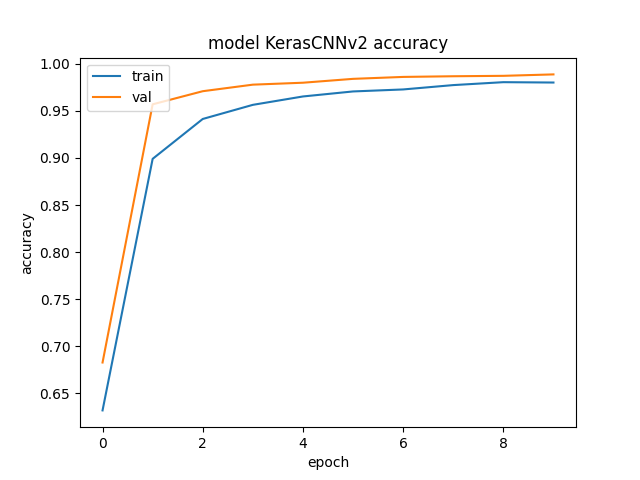
\includegraphics[width=0.6\textwidth]{../Saves/KerasCNNv2/KerasCNNv2_mnist_784_ep10_acc.png}
    \caption{Wykres dokładności w zależności od epoki}
\end{figure}

\begin{figure}[H]
    \centering
    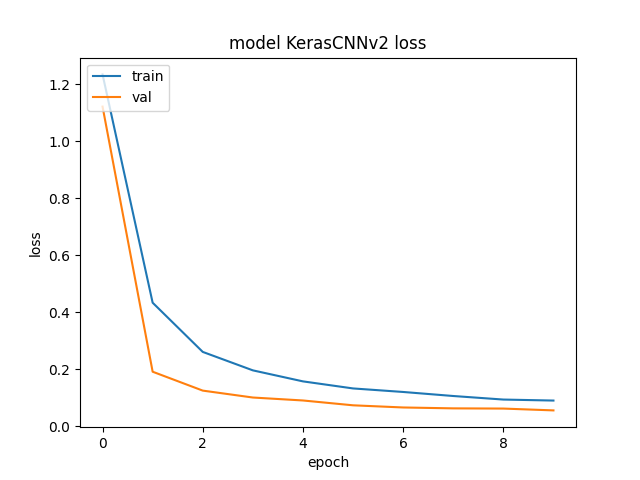
\includegraphics[width=0.6\textwidth]{../Saves/KerasCNNv2/KerasCNNv2_mnist_784_ep10_loss.png}
    \caption{Wykres wartości funkcji straty w zależności od epoki}
\end{figure}

\subsection{Sieć transferowa Tensorflow Keras}

Sieć konwolucyjną transferową zbudowano z użyciem biblioteki tensorflow 
keras oraz modelu transferowego MobileNet klasyfikującego obrazy w 
przestrzeni RGB o rozmiarze przynajmniej $32\times32$px.

Z powodu rozbieżności rozmiarów obrazów, które wymaga sieć MobileNet 
i obrazów należących do baz danych MNIST i podobnych konieczny był 
preprocessing danych wejściowych. Do zastosowanych metod należały:

\begin{itemize}
\item skalowanie obrazów $28\times28$px do rozmiaru $32\times32$px
\item zklonowanie skali szarości na kanały RGB 
\end{itemize}

Dodatkowo by uzyskać jak najlepsze rezultaty na danych nie tylko 
należących do bazy danych, ale stworzyć model, który spełni zadanie 
klasyfikacji możliwie tak dobrze jak człowiek zastosowano 
generowanie nowych danych treningowych w oparciu o dane z bazy z wykorzystaniem:

\begin{itemize}
\item skalowania zawartości obrazu
\item obracania obrazów
\item przesuwania obrazów w osiach X i Y
\end{itemize}

\subsubsection{Przed fine-tuningiem}

\begin{lstlisting}[style=siec]
    Model: "sequential"
    _________________________________________________________________
     Layer (type)                Output Shape              Param #
    =================================================================
     mobilenet_1.00_224 (Functio  (None, 1, 1, 1024)       3228864
     nal)

     flatten (Flatten)           (None, 1024)              0

     dropout (Dropout)           (None, 1024)              0

     dense (Dense)               (None, 512)               524800

     dense_1 (Dense)             (None, 10)                5130

    =================================================================
    Total params: 3,758,794
    Trainable params: 529,930
    Non-trainable params: 3,228,864
    _________________________________________________________________
\end{lstlisting}

Trenowanie before fine-tuning ustawiono na 10 epok:

\begin{figure}[H]
    \centering
    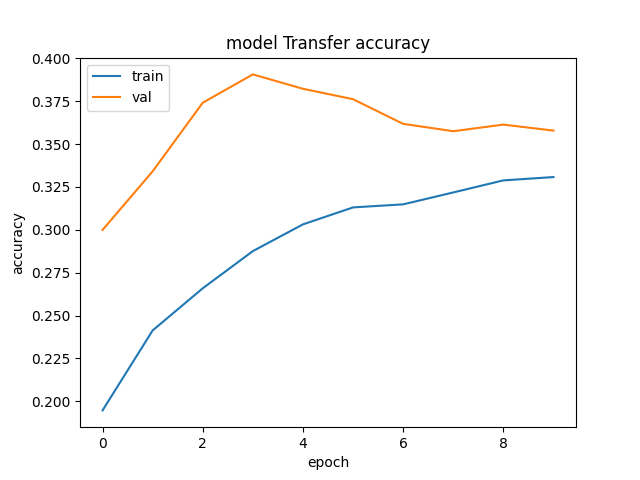
\includegraphics[width=0.6\textwidth]{../Saves/Transfer/Transfer_before_tuning_acc.png}
    \caption{Wykres dokładności w zależności od epoki}
\end{figure}

\begin{figure}[H]
    \centering
    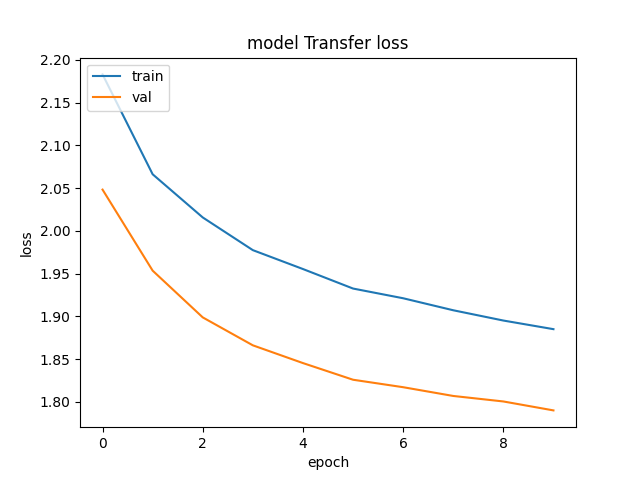
\includegraphics[width=0.6\textwidth]{../Saves/Transfer/Transfer_before_tuning_loss.png}
    \caption{Wykres wartości funkcji straty w zależności od epoki}
\end{figure}

\subsubsection{Fine-tuning}

\begin{lstlisting}[style=siec]
    Model: "sequential"
    _________________________________________________________________
     Layer (type)                Output Shape              Param #
    =================================================================
     mobilenet_1.00_224 (Functio  (None, 1, 1, 1024)       3228864
     nal)

     flatten (Flatten)           (None, 1024)              0

     dropout (Dropout)           (None, 1024)              0

     dense (Dense)               (None, 512)               524800

     dense_1 (Dense)             (None, 10)                5130

    =================================================================
    Total params: 3,758,794
    Trainable params: 3,736,906
    Non-trainable params: 21,888
    _________________________________________________________________
\end{lstlisting}

Trenowanie fine-tuning trwało 100 epok:

\begin{figure}[H]
    \centering
    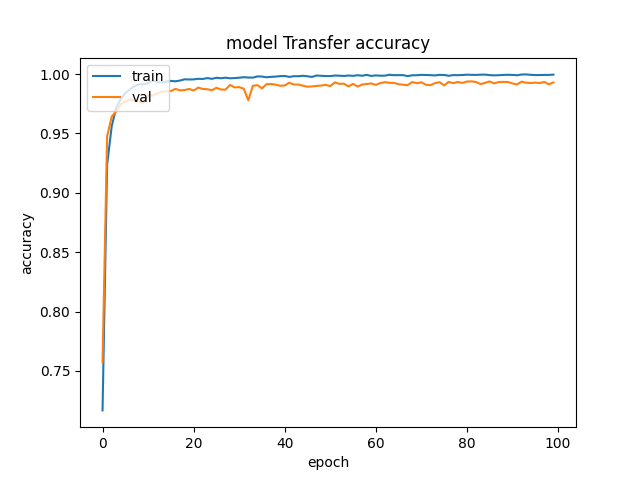
\includegraphics[width=0.6\textwidth]{../Saves/Transfer/Transfer_during_tuning_acc.png}
    \caption{Wykres dokładności w zależności od epoki}
\end{figure}

\begin{figure}[H]
    \centering
    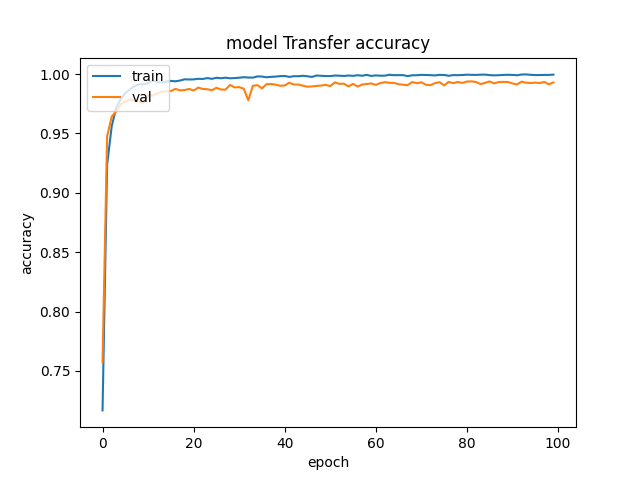
\includegraphics[width=0.6\textwidth]{../Saves/Transfer/Transfer_during_tuning_loss.png}
    \caption{Wykres wartości funkcji straty w zależności od epoki}
\end{figure}


\subsection{Sieć grafowa}
\subsection{K Nearest Neighbours}
Model KNN został zaimplementowany z użyciem biblioteki numpy. Za parametr K 
wybrano wielokrotność liczności zbioru etykiet, 20.



\section{Wyniki}
\subsection{Drzewo decyzyjne}
Przykładowo dla następujących parametrów dla bazy MNIST-784:

\begin{itemize}
    \item max\_depth: 19
    \item max\_features: None
    \item min\_samples\_split: 5
    \item min\_samples\_leaf: 4
    \item criterion: entropy
    \item splitter: random
\end{itemize}
model osiągał skuteczność na danych testowych wynoszącą $0.873$.
\subsection{Las losowy}

Dla następujących parametrów dla bazy MNIST-784:

\begin{itemize}
    \item n\_estimators: 16
    \item max\_depth: 18
    \item max\_features: sqrt
    \item min\_samples\_split: 18
    \item min\_samples\_leaf: 1
    \item criterion: entropy
\end{itemize}
model osiągał skuteczność na danych testowych wynoszącą $0.951$.

\subsection{Własna implementacja Wielowarstwowego perceptronu}
\subsection{Wielowarstwowy perceptron Tensorflow Keras}
\subsection{Sieć konwolucyjna Tensorflow Keras}

Sieć konwolucyjna osiągnęła najwyższą celność na zbiorze testowym równą 0.989 po 
sześciu epochach nie wykazując dużych zmian przy dalszym 
trenowaniu. Jest to wynik dużo lepszy niż w przypadku zwykłego wielowarstwowego 
perceptronu. Dodatkowo proces uczenia tej sieci przebiegał o wiele szybciej niż 
wielowarstwowego perceptronu dzięki warstwom konwolucyjnym, które ograniczyły ilość 
potrzebnych warstw gęstych do jednej.

\subsection{Sieć transferowa Tensorflow Keras}
\subsection{Sieć grafowa}
\subsection{K Nearest Neighbours}

Z powodu długiego czasu predykcji modelu KNN testy wykonano na 10\% zbioru testowego, co odpowiada 1400 danych testowych.
W tej sytuacji model KNN cechował się accuracy na poziomie $0.96$


Z powodu swojej konstrukcji model KNN sprawował się niemal perfekcyjnie 
dla zbioru danych testowych, które przypominały w znacznym stopniu 
dane treningowe. Niestety dla ręcznych rysunków nienależących do 
bazy MNIST-784 model działał dużo gorzej od sieci konwolucyjnej, 
która nie tylko porównuje punkt z danymi treningowymi, lecz 
wynajduje schematy i cechy obrazów, które decydują o 
przynależności do danej klasy. Należy również wspomnieć, 
że z powodu nieporównywalnie większej ilości obliczeń 
koniecznych do wykonania przez model KNN w porównaniu 
do dowolnego innego modelu, podczas gdy proces weryfikacji 
na 14000 danych testowych sieci neuronowych trwał zaledwie 
kilka sekund, weryfikacja modelu KNN zajęła ponad 10 minut dla 1400 danych.

\section{Dyskusja}

Najprawdopodobniej albo... albo szyny, 
które nie były... nie są równe, 
albo po prostu no, tak jak mówiłam we 
wcześniejszym wejściu, ee, yy, szyny... 
szyny były złe... a podwozie... podwozie... 
podwozie... podwozie też było złe. \cite{szyny}

\renewcommand{\refname}{Źródła}
\begin{thebibliography}{100}
    \bibitem{szyny} Wikipedia, 
    \textit{Szyny były złe} 
    \\\url{https://pl.wikipedia.org/wiki/Szyny_by%C5%82y_z%C5%82e}
    \bibitem{bib:2} Super strona,
    \textit{Jest super}
    \\\url{https://www.example.com}
    \bibitem{alicjabogdan} Marek Kubale,
    \textit{Łagodne wprowadzenie do algorytmów}, 2022
\end{thebibliography}

\end{document}


